\documentclass[compress,aspectratio=169]{beamer}
\usepackage{irbookslide}
\usepackage{irilmenau2}
\usepackage{tikz}
\usepackage{url}
\usepackage{ifxetex}
%\RequireXeTeX
\usepackage{fontspec} % zahteva paket euenc
\usepackage{xunicode}
\usepackage{xltxtra}
\usepackage{polyglossia}
\usepackage{minted}
\usepackage[noend]{algorithmic}
\renewcommand{\algorithmicrequire}{\textbf{Input:}}
\renewcommand{\algorithmicensure}{\textbf{Output:}}
\renewcommand{\algorithmiccomment}[1]{\hfill \{\myred{#1}\}}
\usepackage{xcolor,colortbl}
\usepackage{textcomp}
\usepackage{unicode-math}
%\setdefaultlanguage[script=Latin]{serbian}

\title{Analiza algoritama}
\author{\textcopyright \ \ Goodrich, Tamassia, Goldwasser}
\institute{Katedra za informatiku, Fakultet tehničkih nauka, Univerzitet u
Novom Sadu}
\date{2020.}
\subject{Predavanja sa ASP}

\begin{document}

\frame{\titlepage}

\section[Vreme]{Vreme izvršavanja algoritma}
\frame{
  \frametitle{Analiza algoritama}
  \begin{itemize}
    \item algoritam će od nekog ulaza proizvesti neki izlaz \\ \ \\ \ \\
    \item ULAZ $\rightarrow$ ALGORITAM $\rightarrow$ IZLAZ
  \end{itemize}
}
\frame{
  \frametitle{Vreme izvršavanja}
  \begin{itemize}
    \item većina algoritama transformiše objekte na ulazu u objekte na izlazu
    \item \myred{vreme izvršavanja} algoritma obično raste sa veličinom ulaza
    \item teško je izračunati prosečno vreme izvršavanja
    \item posmatraćemo najgori slučaj
    \begin{itemize}
      \item jednostavnije za analizu
      \item ključno za primene kao što su igre, finansije ili robotika
    \end{itemize}
  \end{itemize}
}
\frame{
  \frametitle{Vreme izvršavanja}
  \begin{center}
    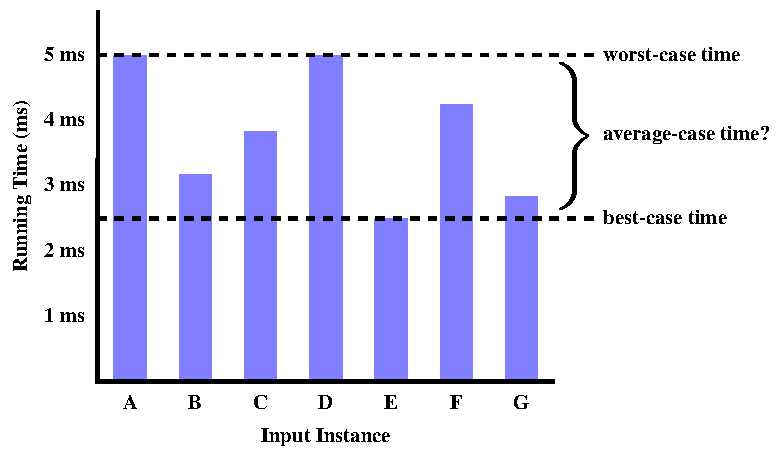
\includegraphics[width=10cm]{asp-01-pic01.pdf}
  \end{center}
}
\frame{
  \frametitle{Eksperimentalno proučavanje algoritama}
  \begin{itemize}
    \item napisati program koji implementira posmatrani algoritam
    \item pokrenuti program za različite veličine i strukturu ulaznih podataka
    \item meriti vreme izvršavanja
    \item analizirati rezultate
  \end{itemize}
}
\begin{frame}[fragile]
  \frametitle{Merenje vremena pomoću sistemskog sata}
\begin{minted}[linenos=false]{python}
from time import time
start_time() = time()
# ... run algorithm ...
end_time = time()
elapsed = end_time - start_time
\end{minted}  
\end{frame}
\frame{
  \frametitle{Analiza rezultata merenja}
  \begin{center}
    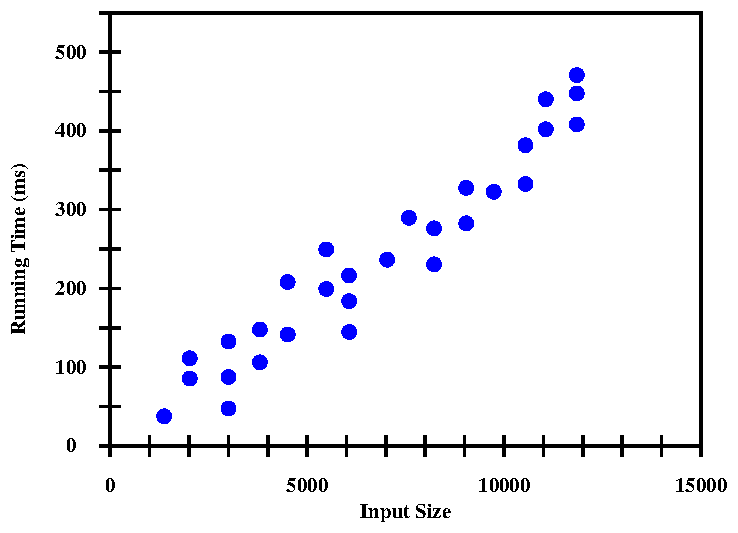
\includegraphics[width=9.5cm]{asp-01-pic02.pdf}
  \end{center}
}
\frame{
  \frametitle{Ograničenja eksperimentalnog pristupa}
  \begin{itemize}
    \item potrebno je implementirati algoritam --- može biti teško
    \item teško je predvideti rezultate za ulaze koji nisu obuhvaćeni
    eksperimentom
    \item za poređenje dva algoritma mora se koristiti identično hardversko
    i softversko okruženje
  \end{itemize}
}
\frame{
  \frametitle{Teorijski pristup}
  \begin{itemize}
    \item koristi se opis algoritma visokog nivoa umesto implementacije
    \item opisuje vreme izvršavanja kao funkciju veličine ulaza --- $n$
    \item uzima u obzir sve moguće ulaze
    \item omogućava procenu brzine algoritma nezavisno od korišćenog hardvera
    ili softvera
  \end{itemize}
}
\frame{
  \frametitle{Pseudokôd}
  \begin{itemize}
    \item opis algoritma visokog nivoa
    \item bolje strukturiran od prirodnog jezika
    \item manje detalja nego u stvarnom programu
    \item sakriva detalje vezane za dizajn programa
    \item poželjna notacija za opisivanje algoritama
  \end{itemize}
}
\section[Pseudokôd]{Pseudokod}
\begin{frame}[fragile]
  \frametitle{Pseudokôd}
  \begin{itemize}
    \item primer: pronalaženje najvećeg broja u nizu
  \end{itemize}
\begin{algorithmic}
\STATE \myred{arrayMax}($A,n$)
\REQUIRE $A$: niz celih brojeva
\REQUIRE $n$: dužina niza
\STATE $currentMax \leftarrow A[0]$
\FOR{$i \leftarrow 1$ \TO $n-1$}
  \IF{$A[i] > currentMax$}
    \STATE $currentMax \leftarrow A[i]$
  \ENDIF
\ENDFOR
\RETURN $currentMax$
\end{algorithmic}
\end{frame}
\begin{frame}[fragile]
  \frametitle{Pseudokôd}
  \begin{itemize}
    \item kontrola toka
    \begin{itemize}
      \item \textbf{if} \ldots \textbf{then} \ldots [\textbf{else}] \textbf{end
      if} 
      \item \textbf{for} \ldots \textbf{do} \ldots \textbf{end for} 
      \item \textbf{while} \ldots \textbf{do} \ldots \textbf{end while} 
      \item \textbf{repeat} \ldots \textbf{until} \ldots 
    \end{itemize}
    \item izrazi 
    \begin{itemize}
      \item $\leftarrow$ dodela vrednosti 
      \item $=$ poređenje vrednosti 
      \item $n^2$ matematička notacija je OK 
    \end{itemize}
    \item vraćanje rezultata
    \begin{itemize}
      \item \textbf{return} vrednost 
    \end{itemize}
  \end{itemize}
\end{frame}

\section[Funkcije]{Sedam važnih funkcija}
\frame{
  \frametitle{Sedam važnih funkcija $_1$}
  \begin{itemize}
    \item \myred{konstantna funkcija}
  \end{itemize}
  $$f(n) = c$$
  \begin{itemize}
    \item osnovna funkcija $g(n)=1$
    \item svaka druga može se prikazati kao $f(n)=c\cdot g(n)$
    \item može da opiše broj koraka potrebnih za neku od osnovnih operacija
    \item npr. sabiranje, dodela vrednosti, poređenje
  \end{itemize}
}
\frame{
  \frametitle{Sedam važnih funkcija $_2$}
  \begin{itemize}
    \item \myred{logaritamska funkcija}
  \end{itemize}
  $$f(n) = \log_b n$$
  \begin{itemize}
    \item za $b>1$
    \item za osnovu logaritma se najčešće koristi 2
    \item 2 se podrazumeva, tj. $\log n = \log_2 n$
    \item podela problema na dva dela: čest princip koji se koristi u
    algoritmima
  \end{itemize}
}
\frame{
  \frametitle{Sedam važnih funkcija $_3$}
  \begin{itemize}
    \item \myred{linearna funkcija}
  \end{itemize}
  $$f(n) = n$$
  \begin{itemize}
    \item kada treba obaviti prostu operaciju nad svakim od $n$ elemenata ulaza
    \item npr. poređenje broja sa svim elementima niza
  \end{itemize}
}
\frame{
  \frametitle{Sedam važnih funkcija $_4$}
  \begin{itemize}
    \item \myred{n-log-n funkcija}
  \end{itemize}
  $$f(n) = n \log n$$
  \begin{itemize}
    \item raste nešto brže od linearne funkcije
    \item i znatno sporije od kvadratne funkcije
    \item npr. najbrže sortiranje $n$ brojeva zahteva $n \log n$ vreme
  \end{itemize}
}
\frame{
  \frametitle{Sedam važnih funkcija $_5$}
  \begin{itemize}
    \item \myred{kvadratna funkcija}
  \end{itemize}
  $$f(n) = n^2$$
  \begin{itemize}
    \item npr. dve ugnježdene petlje 
    \item gde unutrašnja obavlja linearan broj operacija nad elementima ulaza
    \item a spoljna se izvršava linearan broj puta
    \item su proporcionalne sa $n^2$
  \end{itemize}
}
\frame{
  \frametitle{Sedam važnih funkcija $_6$}
  \begin{itemize}
    \item \myred{kubna funkcija}
  \end{itemize}
  $$f(n) = n^3$$
  \begin{itemize}
    \item ređe se javlja od kvadratne, ali 
    \item predstavlja jednu klasu \myred{polinomijalnih} funkcija
  \end{itemize}
  $$ f(n) = a_0 + a_1 n + a_2 n^2 + a_3 n^3 + \ldots + a_d n^d $$
}
\frame{
  \frametitle{Sedam važnih funkcija $_7$}
  \begin{itemize}
    \item \myred{eksponencijalna funkcija}
  \end{itemize}
  $$f(n) = b^n$$
  \begin{itemize}
    \item $b$ je baza
    \item $n$ je eksponent 
    \item često je $b = 2$
    \item najsporija
  \end{itemize}
}
\frame{
  \frametitle{Sedam važnih funkcija}
  \begin{center}
    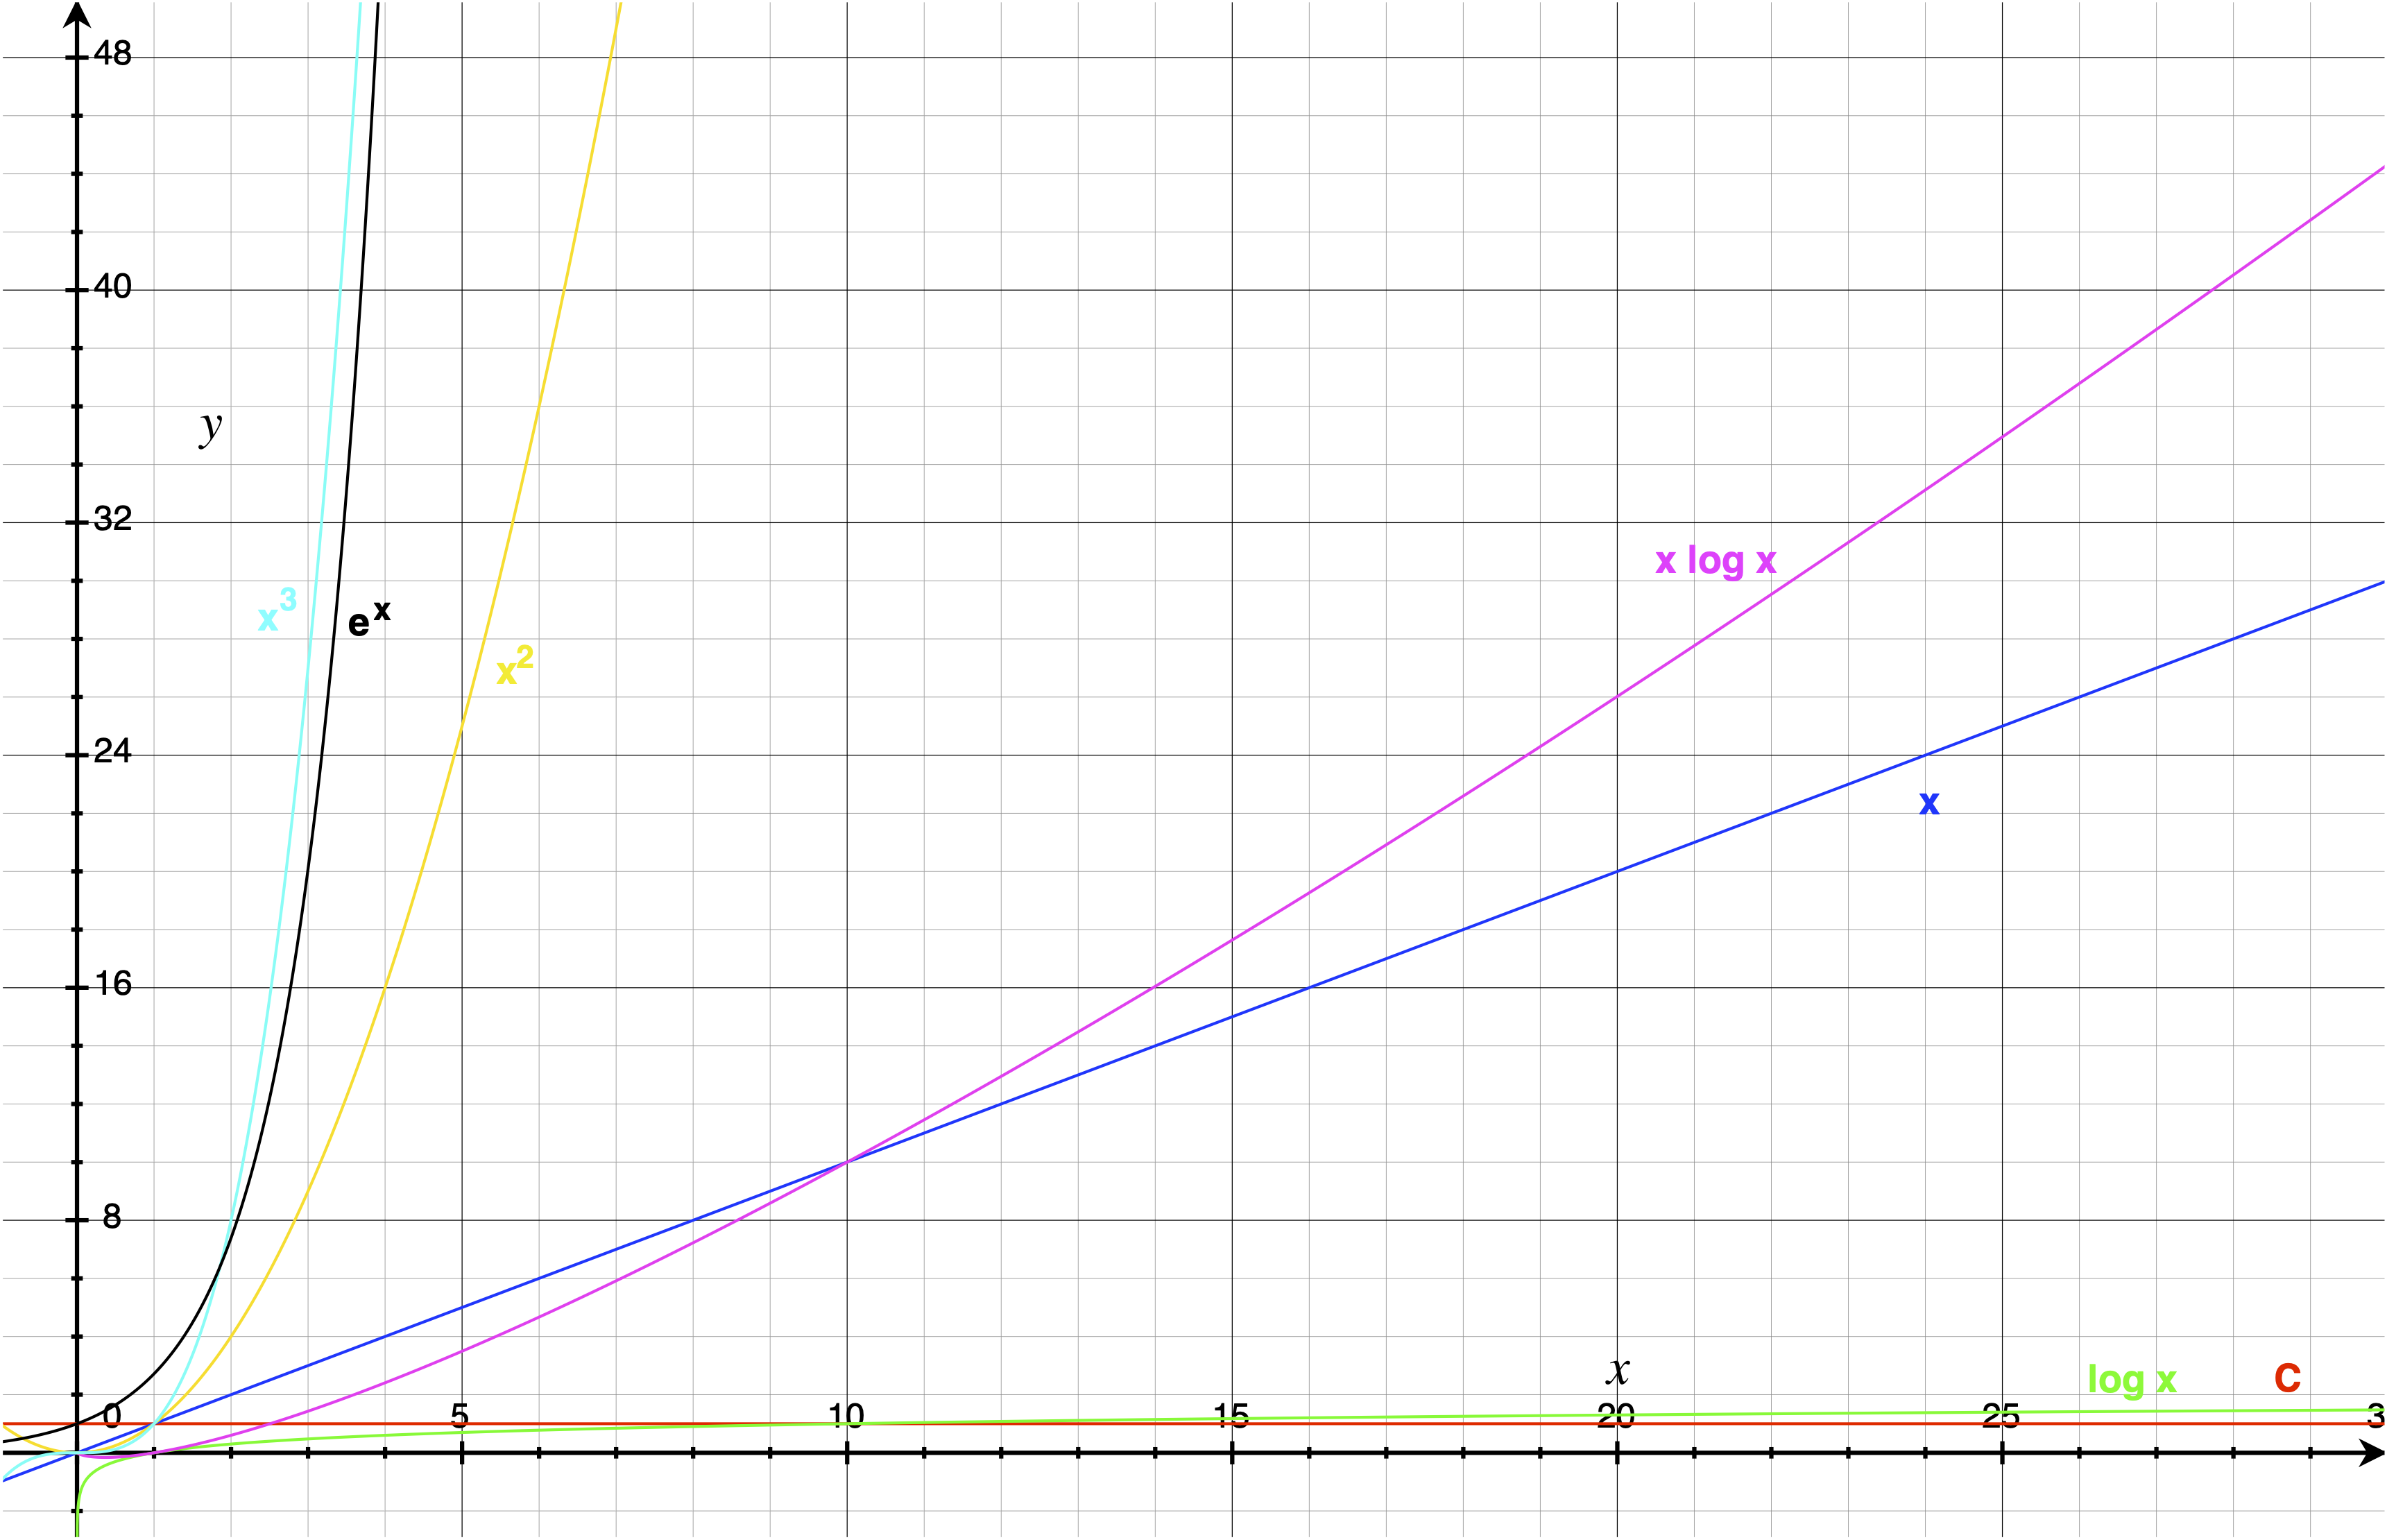
\includegraphics[width=11cm]{7func.png}
  \end{center}
}
\frame{
  \frametitle{Sedam važnih funkcija}
  \begin{center}
    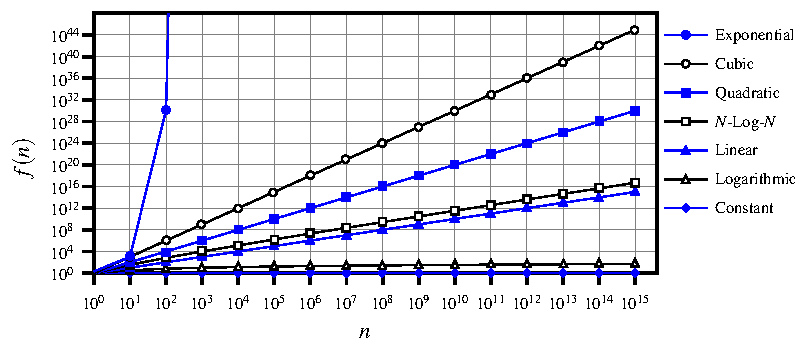
\includegraphics[width=13cm]{asp-01-pic03.pdf}
  \end{center}
}

\section[Procena]{Procena vremena}
\frame{
  \frametitle{Primitivne operacije}
  \begin{itemize}
    \item osnovne operacije koje izvršava algoritam
    \item prikazane u pseudokodu
    \item nezavisne od programskog jezika
    \item troše konstantnu količinu vremena
    \item na primer:
    \begin{itemize}
      \item izračunavanje izraza
      \item dodela vrednosti promenljivoj
      \item pristup elementu niza preko indeksa
      \item poziv funkcije
      \item vraćanje rezultata
    \end{itemize}
  \end{itemize}
}
\begin{frame}[fragile]
  \frametitle{Brojanje primitivnih operacija}
  \begin{itemize}
    \item analizom pseudokoda možemo odrediti maksimalan broj primitivnih
    operacija koje izvršava algoritam kao funkciju veličine ulaza
  \end{itemize}
  \begin{center}
    \begin{tabular}{l|r}
      \textbf{Algoritam} \textit{arrayMax($A, n$)} & \textbf{br. operacija} \\ \hline
      $currentMax \leftarrow A[0]$ & $2$ \\
      \textbf{for} $i \leftarrow 1$ \textbf{to} $n - 1$ \textbf{do} & $2n$ \\
      \ \ \textbf{if} $A[i] > currentMax$ \textbf{then} & $2(n-1)$ \\
      \ \ \ \ $currentMax \leftarrow A[i]$ & $2(n-1)$ \\
      \ \ increment $i$ & $2(n-1)$ \\
      \textbf{return} $currentMax$ & 1 \\ \hline
      \hfill ukupno & $8n-2$
    \end{tabular}
  \end{center}
\end{frame}
\frame{
  \frametitle{Procena vremena izvršavanja}
  \begin{itemize}
    \item algoritam \textbf{arrayMax} izvršava $8n-2$ primitivnih operacija u najgorem slučaju
    \item neka je
    \begin{itemize}
      \item $a$: vreme izvršavanja \textbf{najbrže} primitivne operacije
      \item $b$: vreme izvršavanja \textbf{najsporije} primitivne operacije 
      \item $T(n)$ vreme u najgorem slučaju
    \end{itemize}
    \item tada je
    \begin{itemize}
      \item $a(8n-2) \le T(n) \le b(8n-2)$
      \item $\Rightarrow T(n)$ je ograničena sa dve linearne funkcije!
    \end{itemize}
  \end{itemize}
}
\frame{
  \frametitle{Primer ograničene funkcije}
  \begin{center}
    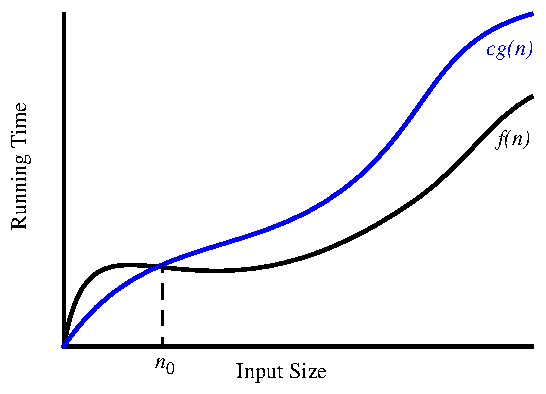
\includegraphics[width=9cm]{asp-01-pic05.pdf}
  \end{center}
}
\frame{
  \frametitle{Porast vremena izvršavanja}
  \begin{itemize}
    \item izmena u hardverskom ili softverskom okruženju 
    \begin{itemize}
      \item menja $T(n)$ za konstantan faktor
      \item ali ne menja brzinu rasta $T(n)$ 
    \end{itemize}
    \item linearni porast vremena izvršavanja $T(n)$ je suštinska osobina algoritma \textbf{arrayMax}
  \end{itemize}
}
\frame{
  \frametitle{Zašto je porast vremena bitan}
  \begin{center}
    \begin{tabular}{l|l|l|l}
      $T(n)$ & \textbf{vreme za n+1} & \textbf{vreme za 2n} & \textbf{vreme za 4n} \\ \hline
      $c \log n$ & $c \log (n+1)$ & $c(\log n + 1)$ & $c(\log n + 2)$ \\
      $cn$ & $c(n+1)$ & $2cn$ & $4cn$ \\
      $cn \log n$ & $\sim c n \log n + cn$ & $2c n \log n + 2cn$ & $4c n \log n + 4cn$ \\
      $cn^2$ & $\sim cn^2+2cn$ & \cellcolor{red!25} $4cn^2$ & $16cn^2$ \\
      $cn^3$ & $\sim cn^3+3cn$ & $8cn^3$ & $64cn^3$ \\
      $c2^n$ & $c2^{n+1}$ & $c2^{2n}$ & $c2^{4n}$ \\
    \end{tabular}
  \end{center}
    \myred{*} za dvostruki ulaz četvorostruko vreme
}
\frame{
  \frametitle{Primer poređenja dva algoritma}
  \begin{itemize}
    \item \myred{insertion sort} je $n^2/4$
    \item \myred{merge sort} je $2n\log n$
    \item sortiramo milion elemenata
    \begin{itemize}
      \item insertion sort $\sim$ \myred{70 sati}
      \item merge sort $\sim$ \myred{40 sekundi}
    \end{itemize}
    \item na 100x bržoj mašini to bi bilo
    \begin{itemize}
      \item insertion sort $\sim$ \myred{40 minuta}
      \item merge sort $\sim$ \myred{0.5 sekundi}
    \end{itemize}
  \end{itemize}
}
\frame{
  \frametitle{Primer poređenja tri algoritma}
  \begin{center}
    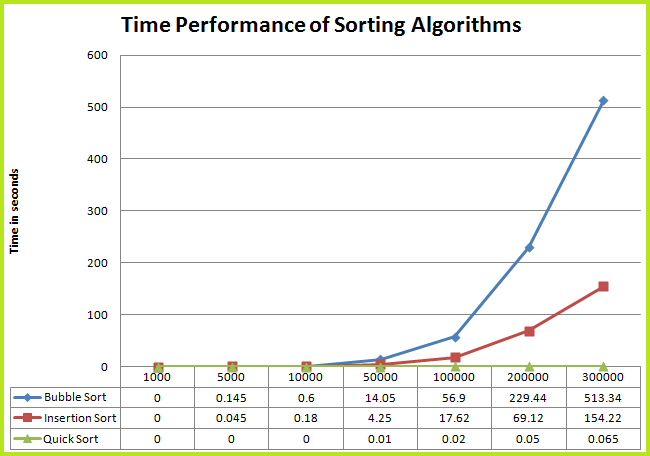
\includegraphics[width=10cm]{asp-01-pic04.png}
  \end{center}
}
\frame{
  \frametitle{Konstantni činioci}
  \begin{itemize}
    \item porast vremena izvršavanja ne zavisi od
    \begin{itemize}
      \item konstantnih činilaca
      \item izraza nižeg reda
    \end{itemize}
    \item na primer
    \begin{itemize}
      \item $10^2n + 10^5$ je linearna funkcija
      \item $10^5n^2 + 10^8n$ je kvadratna funkcija
    \end{itemize}
  \end{itemize}
}
\section[Veliko-O]{Veliko O notacija}
\frame{
  \frametitle{Veliko O notacija}
  \begin{itemize}
    \item ,,Big-Oh``
    \item opisuje granično ponašanje funkcije kada argument raste \\ \ \\
    \item za date $f(n)$ i $g(n)$ kažemo da $f(n)$ je $O(g(n))$ ako postoje pozitivne konstante $c$ i $n_0$ takve da
  \end{itemize}
  $$ f(n) \le cg(n) \;\; \text{za} \;\; n \ge n_0$$
}
\frame{
  \frametitle{Veliko O notacija}
  \begin{itemize}
    \item primer: $2n+10$ je $O(n)$
    \begin{itemize}
      \item $2n+10 \le cn$
      \item $(c-2)n \ge 10$
      \item $n \ge 10/(c-2)$
      \item izaberemo $c=3$ i $n_0=10$
    \end{itemize}
  \end{itemize}
}
\frame{
  \frametitle{Veliko O notacija}
  \begin{itemize}
    \item primer: $n^2$ nije $O(n)$
    \begin{itemize}
      \item $n^2 \le cn$
      \item $n \le c$
      \item ova nejednakost ne može biti zadovoljena jer je $c$ konstanta
    \end{itemize}
  \end{itemize}
}
\frame{
  \frametitle{Još primera}
  \begin{itemize}
    \item $7n-2$ je $O(n)$
    \begin{itemize}
      \item tražimo $c > 0$ i $n_0 \ge 1$ takve da $7n-2 \le cn$ za $n \ge n_0$
      \item ovo je zadovoljeno za $c=7$ i $n_0 = 1$
    \end{itemize}
    \item $3n^3 + 20n^2 + 5$ je $O(n^3)$
    \begin{itemize}
      \item tražimo $c > 0$ i $n_0 \ge 1$ takve da $3n^3 + 20n^2 + 5 \le cn^3$ za $n \ge n_0$
      \item ovo je zadovoljeno za $c=4$ i $n_0 = 21$
    \end{itemize}
    \item $3 \log n + 5$ je $O(\log n)$
    \begin{itemize}
      \item tražimo $c > 0$ i $n_0 \ge 1$ takve da $3 \log n + 5 \le c\log n$ za $n \ge n_0$
      \item ovo je zadovoljeno za $c=8$ i $n_0 = 2$
    \end{itemize}
  \end{itemize}
}
\frame{
  \frametitle{Veliko O i porast vremena}
  \begin{itemize}
    \item veliko O definiše gornju granicu na rast funkcije
    \item tvrdnja $f(n)$ je $O(g(n))$ znači da $f(n)$ ne raste brže od $g(n)$
    \item možemo da koristimo veliko O da rangiramo funkcije po brzini rasta
  \end{itemize}
  \begin{center}
    \begin{tabular}{l|c|c}
      \ & $f(n)$ je $O(g(n))$ & $g(n)$ je $O(f(n))$ \\ \hline
      $g(n)$ raste brže & da & ne \\
      $f(n)$ raste brže & ne & da \\
      jednako brzo rastu & da & da \\
    \end{tabular}
  \end{center}
}
\frame{
  \frametitle{Veliko O: još neka pravila}
  \begin{itemize}
    \item ako je $f(n)$ polinom stepena $d$ tada $f(n)$ je $O(n^d)$, tj.
    \begin{itemize}
      \item možemo zanemariti niže stepene polinoma
      \item možemo zanemariti konstantne koeficijente
    \end{itemize}
    \item koristimo najsporiju moguću klasu funkcija
    \begin{itemize}
      \item kažemo ,,$2n$ je $O(n)$`` umesto ,,$2n$ je $O(n^2)$``
    \end{itemize}
    \item koristimo najjednostavniji izraz koji predstavlja klasu
    \begin{itemize}
      \item kažemo ,,$3n+5$ je $O(n)$`` umesto ,,$3n+5$ je $O(3n)$``
    \end{itemize}
  \end{itemize}
}
\section[Analiza]{Asimptotska analiza}
\frame{
  \frametitle{Asimptotska analiza algoritama}
  \begin{itemize}
    \item asimptotska analiza algoritama određuje vreme izvršavanja u ,,veliko O`` notaciji
    \item kako obaviti asimptotsku analizu
    \begin{itemize}
      \item odredimo broj primitivnih operacija u najgorem slučaju kao funkciju veličine ulaza
      \item izrazimo funkciju u ,,veliko O`` notaciji
    \end{itemize}
    \item primer:
    \begin{itemize}
      \item ustanovimo da \textbf{arrayMax} izvršava najviše $8n-2$ primitivnih operacija
      \item kažemo da je složenost \textbf{arrayMax} algoritma $O(n)$
    \end{itemize}
    \item konstantne činioce i izraze nižeg stepena svakako ne iskazujemo na kraju, pa ih možemo zanemariti kada brojimo primitivne operacije
  \end{itemize}
}
\frame{
  \frametitle{Računanje proseka prefiksa}
  \begin{itemize}
    \item $i$-ti prosek prefiksa niza $X$ je prosek vrednosti prvih $i+1$ elemenata $X$
  \end{itemize}
  $$A[i] = (X[0]+X[1]+\ldots+X[i])/(i+1)$$
  \begin{itemize}
    \item niz $A$ se koristi u finansijskoj analizi
  \end{itemize}
}
\begin{frame}[fragile]
  \frametitle{Računanje proseka prefiksa}
  \begin{itemize}
    \item računanje proseka prefiksa prema definiciji: $O(n^2)$
  \end{itemize}
  \begin{center}
    \begin{tabular}{l|r}
      \textbf{Algoritam} \textit{prefixAverages1(X, n)} & \textbf{br. operacija} \\ \hline
      $A \leftarrow$ novi niz od $n$ integera & $n$ \\
      \textbf{for} $i \leftarrow 0$ \textbf{to} $n - 1$ \textbf{do} & $n$ \\
      \ \ $s \leftarrow X[0]$ & $n$ \\
      \ \ \textbf{for} $j \leftarrow 1$ \textbf{to} $i$ \textbf{do} & $1+2+\ldots+(n-1)$ \\
      \ \ \ \ $s \leftarrow s + X[j]$ & $1+2+\ldots+(n-1)$ \\
      \ \ $A[i] \leftarrow s/(i+1)$ & $n$ \\
      \textbf{return} $A$ & 1
    \end{tabular}
  \end{center}
\end{frame}
\frame{
  \frametitle{Računanje proseka prefiksa}
  \begin{itemize}
    \item složenost \textbf{prefixAverages1} je $O(1+2+\ldots+n)$
    \item suma prvih $n$ prirodnih brojeva je $n(n+1)/2$
    \item $\Rightarrow$ algoritam radi za $O(n^2)$ vreme
  \end{itemize}
  \begin{center}
    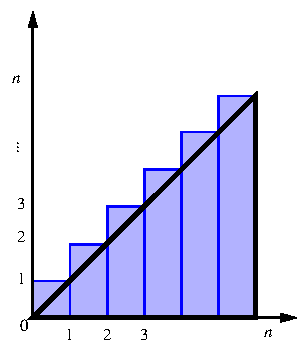
\includegraphics[width=3cm]{asp-01-pic06.pdf}
    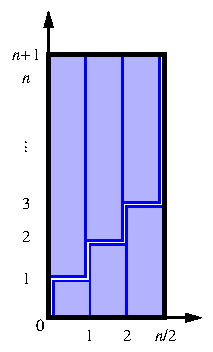
\includegraphics[width=2cm]{asp-01-pic07.pdf}
  \end{center}
}
\begin{frame}[fragile]
  \frametitle{Računanje proseka prefiksa $_2$}
  \begin{itemize}
    \item računanje proseka prefiksa u linearnom vremenu pomoću tekuće sume
  \end{itemize}
  \begin{center}
    \begin{tabular}{l|r}
      \textbf{Algoritam} \textit{prefixAverages2(X, n)} & \textbf{br. operacija} \\ \hline
      $A \leftarrow$ novi niz od $n$ integera & $n$ \\
      $s \leftarrow 0$ & $1$ \\
      \textbf{for} $i \leftarrow 0$ \textbf{to} $n - 1$ \textbf{do} & $n$ \\
      \ \ $s \leftarrow s + X[i]$ & $n$ \\
      \ \ $A[i] \leftarrow s/(i+1)$ & $n$ \\
      \textbf{return} $A$ & 1
    \end{tabular}
  \end{center}
\end{frame}
\frame{
  \frametitle{Šta nam treba od matematike}
  \begin{itemize}
    \item tehnike izvođenja dokaza
    \item verovatnoća
    \item redovi
    \item logaritmi
    \begin{itemize}
      \item $\log_b(xy) = \log_bx+\log_by$
      \item $\log_b(x/y) = \log_bx-\log_by$
      \item $\log_b(xa) = a\log_bx$
      \item $\log_ba = log_xa/\log_xb$
    \end{itemize}
    \item eksponencijalne funkcije
    \begin{itemize}
      \item $a^{b+c} = a^b a^c$
      \item $a^{bc} = (a^b)^c$
      \item $a^b/a^c = a^{b-c}$
      \item $b = a\log_ab$
      \item $b^c = a^{c\log_ab}$
    \end{itemize}
  \end{itemize}
}
\frame{
  \frametitle{Rođaci velikog O}
  \begin{itemize}
    \item $\Omega$: veliko Omega
    \begin{itemize}
      \item $f(n)$ je $\Omega(g(n))$ ako postoje $c>0$ i $n_0\ge 1$ takvi da $f(n)\ge cg(n)$ za $n\ge n_0$
    \end{itemize}
    \item $\Theta$: veliko Teta
    \begin{itemize}
      \item $f(n)$ je $\Theta(g(n))$ ako postoje $c_1>0$ $c_2>0$ i $n_0\ge 1$ takvi da $c_1g(n) \le f(n) \le c_2g(n)$ za $n\ge n_0$
    \end{itemize}
  \end{itemize}
}
\frame{
  \frametitle{Rođaci velikog O}
  \begin{itemize}
    \item veliko O
    \begin{itemize}
      \item $f(n)$ je $O(g(n))$ ako je $f(n)$ asimptotski \myred{manje ili jednako} $g(n)$
    \end{itemize}
    \item veliko $\Omega$
    \begin{itemize}
      \item $f(n)$ je $\Omega(g(n))$ ako je $f(n)$ asimptotski \myred{veće ili jednako} $g(n)$
    \end{itemize}
    \item veliko $\Theta$
    \begin{itemize}
      \item $f(n)$ je $\Theta(g(n))$ ako je $f(n)$ asimptotski \myred{jednako} $g(n)$
    \end{itemize}
  \end{itemize}
}
\frame{
  \frametitle{Primeri sa O, $\Omega$, $\Theta$}
  \begin{itemize}
    \item $5n^2$ je $\Omega(n^2)$
    \begin{itemize}
      \item $f(n)$ je $\Omega(g(n))$ ako postoje $c>0$ i $n_0\ge 1$ takvi da $f(n)\ge cg(n)$ za $n\ge n_0$
      \item rešenje: $c = 5$ i $n_0 = 1$
    \end{itemize}
    \item $5n^2$ je $\Omega(n)$
    \begin{itemize}
      \item $f(n)$ je $\Omega(g(n))$ ako postoje $c>0$ i $n_0\ge 1$ takvi da $f(n)\ge cg(n)$ za $n\ge n_0$
      \item rešenje: $c = 1$ i $n_0 = 1$
    \end{itemize}
    \item $5n^2$ je $\Theta(n^2)$
    \begin{itemize}
      \item $f(n)$ je $\Theta(g(n))$ ako je $\Omega(n^2)$ i $O(n^2)$; prvi uslov smo proverili a drugi je ispunjen za 
      \item $c = 5$ i $n_0 = 1$
    \end{itemize}
  \end{itemize}
}
\end{document}
